\documentclass[12pt, a4paper]{report}

% Packages :

\usepackage[french]{babel}
\usepackage[utf8]{inputenc}
\usepackage[T1]{fontenc}
\usepackage[pdftex, pdfauthor={Bacomathiques}]{hyperref}
\usepackage{sectsty}
\usepackage[explicit]{titlesec}
\usepackage{xcolor}
\usepackage{amsmath}
\usepackage{amssymb}
\usepackage{amsthm}
\usepackage{fourier}
\usepackage{titlesec}
\usepackage{fancyhdr}
\usepackage{catchfilebetweentags}
\usepackage[french, capitalise, noabbrev]{cleveref}
\usepackage[fit, breakall]{truncate}
\usepackage[margin=3cm]{geometry}
\usepackage{tocloft}
\usepackage{tikz}
\usepackage{tocloft}
\usepackage{microtype}
\usepackage{listings}
\usepackage{tabularx}
\usepackage{calc}
\usepackage[export]{adjustbox}
\usepackage[most]{tcolorbox}
\usepackage{standalone}
\usepackage{xlop}
\usepackage{etoolbox}
\usepackage{environ}

\usetikzlibrary{arrows.meta}
\usetikzlibrary{trees}

% Paramètres :

\author{Bacomathiques}
\definecolor{graphe}{HTML}{93c9ff}
\setcounter{MaxMatrixCols}{12}
\setlength{\parindent}{0pt}
\setlength{\fboxsep}{0pt}
%\pdfsuppresswarningpagegroup=1

% Code :

\lstdefinestyle{style}{
	backgroundcolor=\color{white},
	commentstyle=\em\color[HTML]{999988},
	keywordstyle=\bfseries,
	identifierstyle=\normalfont,
	stringstyle=\color[rgb]{0.87, 0.07, 0.27},
	basicstyle=\ttfamily\color{black},
	breakatwhitespace=false,
	breaklines=true,
	captionpos=b,
	keepspaces=true,
	numbers=left,
	numbersep=5pt,
	showspaces=false,
	showstringspaces=false,
	showtabs=false,
	tabsize=2,
	numbers=none
}

\lstset{style=style}
\lstset{
	literate=
	{á}{{\'a}}1
	{à}{{\`a}}1
	{ã}{{\~a}}1
	{é}{{\'e}}1
	{ê}{{\^e}}1
	{í}{{\'i}}1
	{ó}{{\'o}}1
	{õ}{{\~o}}1
	{ú}{{\'u}}1
	{ü}{{\"u}}1
	{ç}{{\c{c}}}1
}

\lstset{
	framextopmargin=10pt,
	framexrightmargin=10pt,
	framexbottommargin=10pt,
	framexleftmargin=10pt,
	xleftmargin=10pt,
	xrightmargin=10pt,
}

% Couleurs :

\definecolor{title}{HTML}{912c21}
\definecolor{section}{HTML}{1c567d}
\definecolor{subsection}{HTML}{2980b9}

\definecolor{rule}{HTML}{c4c4c4}

\definecolor{formula}{HTML}{ebf3fb}
\definecolor{formula-left}{HTML}{3583d6}

\definecolor{tip}{HTML}{dcf3d8}
\definecolor{tip-left}{HTML}{26a65b}

\definecolor{demonstration}{HTML}{fff8de}
\definecolor{demonstration-left}{HTML}{f1c40f}

\definecolor{exercise}{HTML}{e0f2f1}
\definecolor{exercise-left}{HTML}{009688}

\definecolor{correction}{HTML}{e0f7fa}
\definecolor{correction-left}{HTML}{00bcd4}

\definecolor{toc}{HTML}{fceae9}
\definecolor{toc-left}{HTML}{e74c3c}
\definecolor{toc-dark}{HTML}{87281f}

% Titres :

\renewcommand{\thesection}{\Roman{section} - }
\renewcommand{\thesubsection}{\arabic{subsection}. }

\newcommand{\sectionstyle}{\normalfont\LARGE\bfseries\color{section}}
\titleformat{\section}{\sectionstyle}{\thesection #1}{0pt}{}
\titleformat{name=\section, numberless}{\sectionstyle}{#1}{0pt}{}

\newcommand{\subsectionstyle}{\normalfont\Large\bfseries\color{subsection}}
\titleformat{\subsection}{\subsectionstyle}{\thesubsection #1}{0pt}{}
\titleformat{name=\subsection, numberless}{\subsectionstyle}{#1}{0pt}{}

\titlelabel{\thetitle\ }

% Table des matières :

\addto\captionsfrench{\renewcommand\contentsname{}}
\renewcommand{\cftsecpagefont}{\color{toc-dark}}
\renewcommand{\cftsubsecpagefont}{\color{toc-dark}}
\renewcommand{\cftsecleader}{\cftdotfill{\cftdotsep}}
\renewcommand{\cftsecfont}{\bfseries}
\renewcommand{\cftsecpagefont}{\bfseries\color{toc-dark}}
\setlength{\cftbeforetoctitleskip}{0pt}
\setlength{\cftaftertoctitleskip}{0pt}
\setlength{\cftsecindent}{0pt}
\setlength{\cftsubsecindent}{20pt}
\setlength{\cftsubsecnumwidth}{20pt}

% Commandes :

\newcommand{\newpar}{\\[\medskipamount]}
\newcommand{\lesson}[3]{%
	\newcommand{\level}{#1}%
	\newcommand{\id}{#2}%
	\hypersetup{pdftitle={#3}}
	\begin{center}%
		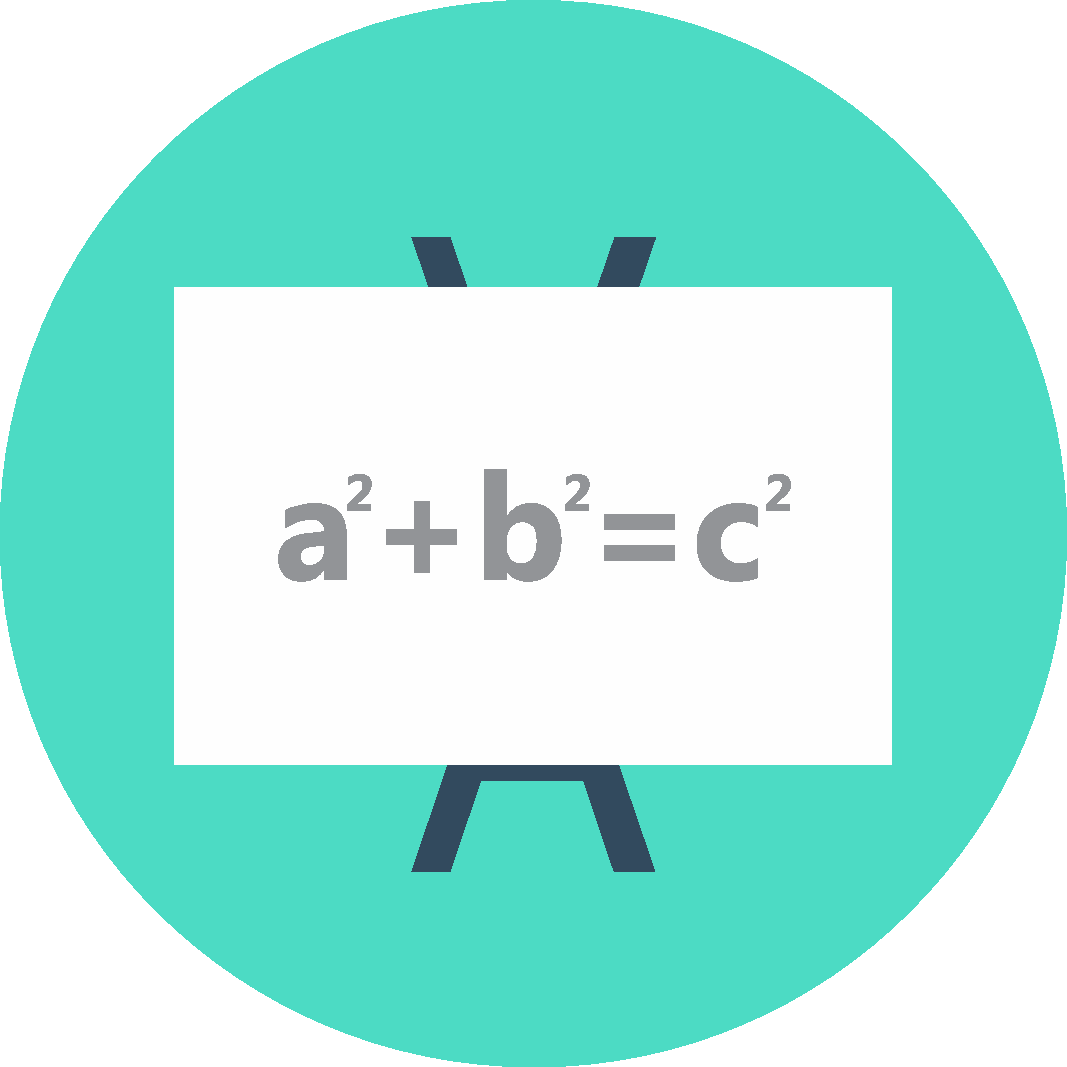
\includegraphics[width=150px]{\imagespath/bacomathiques}%
		
		\vspace{30pt}%
		{\Huge\color{title} #3}%
		
		\vspace{10pt}%
		{Bacomathiques --- \href{https://bacomathiqu.es/cours/#1/#2}{\color{section} https://bacomathiqu.es}}%
		
		\vspace{20pt}%
	\end{center}%
	\begin{toc}
		\tableofcontents%
	\end{toc}
	\thispagestyle{empty}%
	\newpage%
	\setcounter{page}{1}%
}
\newcommand{\imagespath}{../../images}
\newcommand{\lessonimagespath}{\imagespath/lessons/\level/\id/}
\newcommand{\includelatexpicture}[2][\textwidth - 100pt]{%
	\begin{center}%
		\resizebox{#1}{!}{%
			\input{\lessonimagespath#2}%
		}%
	\end{center}%
	\medskip%
}
\newcommand{\includeimage}[1]{%
	\begin{center}%
		\includegraphics{\lessonimagespath#1}%
	\end{center}%
	\medskip%
}
\newcommand{\includerepresentation}[1]{%
	\begin{center}%
		\setlength{\fboxrule}{0.5pt}%
		\href{https://www.geogebra.org/m/#1}{\includegraphics[width=\textwidth-1pt,fbox]{\lessonimagespath#1}}%
	\end{center}%
}
\newcommand{\floor}[1]{\lfloor #1 \rfloor}

\makeatletter
\newcommand\inputcontent{\@ifstar{\inputcontent@star}{\inputcontent@nostar}}
\newcommand{\inputcontent@star}[1]{%
	\ExecuteMetaData[#1]{content}%
}
\newcommand{\inputcontent@nostar}[1]{%
	\newpage%
	\inputcontent@star{#1}%
}
\makeatother

\let\oldsection\section
\renewcommand\section{\clearpage\oldsection}
\newcommand{\contentwidth}[1][medium]{}

% En-têtes :

\pagestyle{fancy}

\renewcommand{\sectionmark}[1]{\markboth{\thesection \ #1}{}}

\fancyhead[R]{\truncate{0.23\textwidth}{\color{title}\thepage}}
\fancyhead[L]{\truncate{0.73\textwidth}{\color{title}\leftmark}}
\fancyfoot[C]{\scriptsize \href{https://bacomathiqu.es/cours/\level/\id}{\texttt{bacomathiqu.es}}}

\makeatletter
\patchcmd{\f@nch@head}{\rlap}{\color{rule}\rlap}{}{}
\patchcmd{\headrule}{\hrule}{\color{rule}\hrule}{}{}
\makeatother

% Environnements :

\newenvironment{nosummary}{}{}
\newcommand{\tcolorboxtitle}[2]{\setlength{\fboxsep}{2.5pt}\hspace{-10pt}\colorbox{#1-left}{\hspace{8pt}\MakeUppercase{#2} \hspace{2pt} \includegraphics[height=0.8em]{\imagespath/bubbles/#1}\hspace{5pt}}}
\newcommand{\tcolorboxsubtitle}[2]{\ifstrempty{#2}{}{\textcolor{#1-left}{\large#2}\\[\medskipamount]}}
\tcbset{
	frame hidden,
	boxrule=0pt,
	boxsep=0pt,
	enlarge bottom by=8.5pt,
	enhanced jigsaw,
	boxed title style={sharp corners,boxrule=0pt,coltitle={white},titlerule=0pt},
	fonttitle=\fontsize{6pt}{6pt}\bfseries\boldmath,
	top=10pt,
	right=10pt,
	bottom=10pt,
	left=10pt,
	arc=0pt,
	outer arc=0pt,
}
\newtcolorbox{toc}[1][]{
	colback=toc,
	borderline west={3pt}{0pt}{toc-left},
	title=\tcolorboxtitle{toc}{Table des matières},
	colbacktitle=toc,
	before upper={\tcolorboxsubtitle{toc}{#1}}
}
\newtcolorbox{formula}[1][]{
	colback=formula,
	borderline west={3pt}{0pt}{formula-left},
	title=\tcolorboxtitle{formula}{À retenir},
	colbacktitle=formula,
	before upper={\tcolorboxsubtitle{formula}{#1}}
}
\newtcolorbox{tip}[1][]{
	colback=tip,
	borderline west={3pt}{0pt}{tip-left},
	title=\tcolorboxtitle{tip}{À lire},
	colbacktitle=tip,
	before upper={\tcolorboxsubtitle{tip}{#1}}
}
\newtcolorbox{demonstration}[1][]{
	colback=demonstration,
	borderline west={3pt}{0pt}{demonstration-left},
	title=\tcolorboxtitle{demonstration}{Démonstration},
	colbacktitle=demonstration,
	before upper={\tcolorboxsubtitle{demonstration}{#1}}
}

\NewEnviron{whitetabularx}[1]{%
	\renewcommand{\arraystretch}{2.5}
	\colorbox{white}{%
		\begin{tabularx}{\textwidth}{#1}%
			\BODY%
		\end{tabularx}%
	}%
}

% Longueurs :

\newlength{\espacetitreliste}
\setlength{\espacetitreliste}{-16pt}
\newcommand{\entretitreetliste}{\vspace{\espacetitreliste}}

\begin{document}
	%<*content>
	\lesson{terminale}{suites}{Chapitre I -- Les suites}

	\section{Définitions}

	\subsection{Suites numériques}

	Pour rappel, on appelle \textbf{suite} une fonction (et plus précisément application) de $\mathbb{N}$ dans $\mathbb{R}$ : cette fonction va prendre des éléments de l'ensemble de départ $\mathbb{N}$ et va les amener dans l'ensemble d'arrivée $\mathbb{R}$.

	\begin{formula}[Définition]
		Il y a plusieurs manières de définir une suite :
		\begin{itemize}
			\item \textbf{Par récurrence :} On donne le premier terme de la suite ainsi que le terme au rang $n+1$.
			\item \textbf{Par son terme général :} On donne le $n$-ième terme de la suite en fonction de $n$.
		\end{itemize}
	\end{formula}

	\textbf{Attention !} Bien que ces deux modes de génération soient les principaux, il en existe d'autres : algorithme, motifs géométriques, ...

	\begin{tip}[Exemple]
		On définit les suites $(u_n)$ et $(v_n)$ ainsi :
		\begin{itemize}
			\item $u_n = n$ pour tout $n \in \mathbb{N}$ ($(u_n)$ est définie par son terme général).
			\item $(v_n) = \begin{cases} v_0 = 0 \\ v_{n+1} = v_n + 1 \text{ pour tout } n \geq 1 \end{cases}$ ($(v_n)$ est définie par récurrence).
		\end{itemize}
		On remarque que bien que définies différemment, $(u_n)$ et $(v_n)$ sont égales.
	\end{tip}

	\subsection{Sens de variation}

	\begin{formula}[Définition]
		Soit $(u_n)$ une suite.
		\begin{itemize}
			\item $(u_n)$ est \textbf{croissante} si on a $u_{n+1} \geq u_n$ (ou $u_{n+1} - u_n \geq 0$) pour tout $n \in \mathbb{N}$.
			\item $(u_n)$ est \textbf{décroissante} si on a $u_{n+1} \leq u_n$ (ou $u_{n+1} - u_n \leq 0$) pour tout $n \in \mathbb{N}$.
			\item $(u_n)$ est dite \textbf{constante} s'il existe $c \in \mathbb{R}$ tel que $u_n = c$ pour tout $n \in \mathbb{N}$.
		\end{itemize}
	\end{formula}

	Si une suite est croissante ou décroissante et ne change pas de variation, alors elle est dite \textbf{monotone}.

	\subsection{Convergence et divergence}

	\begin{formula}[Convergence]
		On dit qu'une suite $(u_n)$ \textbf{converge} vers un réel $\ell$ quand $n$ tend vers $+\infty$ si :
		\newpar
		Pour tout $\epsilon > 0$, l'intervalle ouvert $]\ell-\epsilon, \ell+\epsilon[$, contient tous les termes de la suite $(u_n)$ à partir d'un certain rang. On note alors : $\lim\limits_{n \rightarrow +\infty} u_n = \ell$.
	\end{formula}

	\begin{tip}
		Cette définition est un peu abstraite mais elle signifie simplement que $u_n$ se rapproche autant que l'on veut de $\ell$ pourvu que $n$ soit assez grand.
	\end{tip}

	\textbf{Attention !} Il est tout à fait possible que la suite $(u_n)$ converge vers un réel $\ell$ mais ne soit jamais égal à $\ell$.

	\begin{formula}[Divergence vers $+\infty$]
		On dit qu'une suite $(v_n)$ \textbf{diverge} vers $+\infty$ quand $n$ tend vers $+\infty$ si :
		\newpar
		Pour tout $A > 0$, il existe un rang $N$ tel que pour tout $n \geq N$, $v_n > A$. On note alors : $\lim\limits_{n \rightarrow +\infty} u_n = +\infty$.
	\end{formula}

	Il existe une définition similaire pour la divergence vers $-\infty$.

	\begin{tip}[Divergence vers $-\infty$]
		Dire que $(v_n)$ \textbf{diverge} vers $-\infty$ signifie que :
		\newpar
		Pour tout $A > 0$, il existe un rang $N$ tel que pour tout $n \geq N$, $v_n < -A$. On note alors : $\lim\limits_{n \rightarrow +\infty} u_n = -\infty$.
	\end{tip}

	\begin{tip}
		À noter que l'on n'étudie les limites des \textbf{suites} que quand $n$ tend vers $+\infty$, et qu'il est possible qu'une suite n'admette pas de limite. On dit alors que cette suite \textbf{diverge}. Par contre, si une suite converge vers une limite, alors cette limite est \textbf{unique}.
	\end{tip}

	\section{Calcul de limites}

	\subsection{Limites de suites de référence}

	Nous allons donner quelques suites ``classiques'' avec leur limite en $+\infty$ :

	\begin{formula}[Limites de suites usuelles]
		\begin{whitetabularx}{|X|X|}
			\hline
			\textbf{Suite} & \textbf{Limite quand $n$ tend vers $+\infty$} \\
			\hline
			$(\sqrt{n})$ & $+\infty$ \\
			\hline
			$(n)$ & $+\infty$ \\
			\hline
			$(n^k)$, pour $k \in \mathbb{N}^*$ & $+\infty$ \\
			\hline
			$\left(\frac{1}{\sqrt{n}}\right)$ & $0$ \\
			\hline
			$\left(\frac{1}{n}\right)$ & $0$ \\
			\hline
			$\left(\frac{1}{n^k}\right)$, pour $k \in \mathbb{N}^*$ & $0$ \\
			\hline
		\end{whitetabularx}
	\end{formula}

	Nous allons désormais donner la limite d'une catégorie de suite très importante en mathématiques : celle des \textbf{suites géométriques}. Ainsi :

	\begin{formula}[Limite de suites géométriques]
		Soit $(v_n)$ une suite définie pour tout $n \in \mathbb{N}$ par $v_n = q^n$ (où $q$ est un nombre réel). Alors, on peut donner la limite de la suite $(v_n)$ en fonction de $q$ :
		\newpar
		\begin{whitetabularx}{|X|l|l|l|l|l|}
			\hline
			\multicolumn{5}{|l|}{\textbf{Limite d'une suite géométrique}} \\
			\hline
			Si on a... & $-1 < q < 1$ & $1 < q$ & $q \leq -1$ & $q = 1$ \\
			\hline
			Alors la suite $(v_n)$ a pour limite... & $0$ & $+\infty$ & Pas de limite & $1$ \\
			\hline
		\end{whitetabularx}
	\end{formula}

	\begin{tip}
		Le réel $q$ est la \textbf{raison} de la suite : si $q > 1$, $(v_n)$ est strictement croissante, si $0 < q < 1$, $(v_n)$ est strictement décroissante et si $q = 1$ ou $0$, $(v_n)$ est constante.
	\end{tip}

	\subsection{Opérations sur les limites}

	Dans tout ce qui suit, $(u_n)$ et $(v_n)$ sont deux suites. Ces tableaux sont à connaître et sont requis pour pouvoir travailler sur les limites.

	\begin{formula}[Limite d'une somme]
		\begin{whitetabularx}{|X|l|l|l|l|l|l|}
			\hline
			\multicolumn{7}{|l|}{\textbf{Limite d'une somme}} \\
			\hline
			Si la limite de $(u_n)$ quand $n$ tend vers $+\infty$ est... & $\ell$ & $\ell$ & $\ell$ & $+\infty$ & $-\infty$ & $+\infty$ \\
			\hline
			Et la limite de $(v_n)$ quand $n$ tend vers $+\infty$ est... & $\ell'$ & $+\infty$ & $-\infty$ & $+\infty$ & $-\infty$ & $-\infty$ \\
			\hline
			Alors la limite de $(u_n + v_n)$ quand $n$ tend vers $+\infty$ est... & $\ell + \ell'$ & $+\infty$ & $-\infty$ & $+\infty$ & $-\infty$ & \textbf{?} \\
			\hline
		\end{whitetabularx}
	\end{formula}

	\begin{formula}[Limite d'un produit]
		\begin{whitetabularx}{|X|l|l|l|l|l|l|l|l|l|}
			\hline
			\multicolumn{10}{|l|}{\textbf{Limite d'un produit}} \\
			\hline
			Si la limite de $(u_n)$ quand $n$ tend vers $+\infty$ est... & $\ell$ & $\ell > 0$ & $\ell > 0$ & $\ell < 0$ & $\ell < 0$ & $+\infty$ & $+\infty$ & $-\infty$ & $0$ \\
			\hline
			Et la limite de $(v_n)$ quand $n$ tend vers $+\infty$ est... & $\ell'$ & $+\infty$ & $-\infty$ & $+\infty$ & $-\infty$ & $+\infty$ & $-\infty$ & $-\infty$ & $\pm \infty$ \\
			\hline
			Alors la limite de $(u_n \times v_n)$ quand $n$ tend vers $+\infty$ est... & $\ell \times \ell'$ & $+\infty$ & $-\infty$ & $-\infty$ & $+\infty$ & $+\infty$ & $-\infty$ & $+\infty$ & \textbf{?} \\
			\hline
		\end{whitetabularx}
	\end{formula}

	\begin{formula}[Limite d'un quotient]
		\begin{whitetabularx}{|X|l|l|l|l|l|l|l|l|l|}
			\hline
			\multicolumn{10}{|l|}{\textbf{Limite d'un quotient}} \\
			\hline
			Si la limite de $(u_n)$ quand $n$ tend vers $+\infty$ est... & $\ell$ & $\ell$ & $+\infty$ & $+\infty$ & $-\infty$ & $-\infty$ & $\pm \infty$ & $\ell$ & $0$ \\
			\hline
			Et la limite de $(v_n)$ quand $n$ tend vers $+\infty$ est... & $\ell' \neq 0$ & $\pm \infty$ & $\ell' > 0$ & $\ell' < 0$ & $\ell' > 0$ & $\ell' < 0$ & $\pm \infty$ & $0^+_-$ & $0$ \\
			\hline
			Alors la limite de $\left(\frac{u_n}{v_n}\right)$ quand $n$ tend vers $+\infty$ est... & $\frac{\ell}{\ell'}$ & $0$ & $+\infty$ & $-\infty$ & $-\infty$ & $+\infty$ & \textbf{?} & $\pm \infty$ & \textbf{?} \\
			\hline
		\end{whitetabularx}
	\end{formula}

	\begin{tip}[Formes indéterminées]
		À noter qu'il n'existe que 4 formes indéterminées : ``$+\infty - \infty$'', ``$0 \times \pm \infty$'', ``$\frac{\pm \infty}{\pm \infty}$'' et ``$\frac{0}{0}$''.
	\end{tip}

	\subsection{Majoration, minoration et bornes}

	\begin{formula}[Définition]
		Soient une suite $(u_n)$ et deux réels $m$ et $M$ :
		\begin{itemize}
			\item On dit que $m$ est un \textbf{minorant} de $(u_n)$ si pour tout $n$ : $u_n > m$.
			\item On dit que $M$ est un \textbf{majorant} de $(u_n)$ si pour tout $n$ : $u_n < M$.
			\item On dit que $(u_n)$ est \textbf{bornée} si elle est à la fois majorée et minorée.
		\end{itemize}
	\end{formula}

	\begin{formula}[Théorème]
		\entretitreetliste
		\begin{itemize}
			\item Si $(u_n)$ est croissante et est majorée, alors elle est convergente. Si elle n'est pas majorée, $(u_n)$ diverge vers $+\infty$.
			\item Si $(u_n)$ est décroissante et est minorée, alors elle est convergente. Si elle n'est pas minorée, $(u_n)$ diverge vers $-\infty$.
		\end{itemize}
	\end{formula}

	\begin{demonstration}
		Il faut savoir montrer que toute suite croissante et non majorée diverge vers $+\infty$. C'est ce que nous allons faire ici. Soit donc $(u_n)$ une telle suite. Soit $A > 0$, on cherche un rang $N$ tel que pour tout $n \geq N$, $u_n > A$.
		\newpar
		Or, comme $(u_n)$ est non majorée, il existe $N$ tel que $u_N > A$. De plus, comme $(u_n)$ est croissante, alors $A < u_N \leq u_{N+1} \leq u_{N+2} \leq \dots$
		\newpar
		Donc on a bien trouvé notre rang $N$ vérifiant la définition de la divergence vers $+\infty$.
	\end{demonstration}

	\begin{tip}
		Toute suite convergente est également bornée.
	\end{tip}

	\subsection{Comparaisons et encadrements}

	\begin{formula}[Théorèmes de comparaison]
		Soient deux suites $(u_n)$ et $(v_n)$ telles que $u_n < v_n$ à partir d'un certain rang $N$. On a :
		\begin{itemize}
			\item Si $\lim\limits_{n \rightarrow +\infty} u_n = +\infty$, alors $\lim\limits_{n \rightarrow +\infty} v_n = +\infty$.
			\item Si $\lim\limits_{n \rightarrow +\infty} v_n = -\infty$, alors $\lim\limits_{n \rightarrow +\infty} u_n = -\infty$.
			\item Si $\lim\limits_{n \rightarrow +\infty} u_n = \ell$ et $\lim\limits_{n \rightarrow +\infty} v_n = \ell'$ alors $\ell < \ell'$.
		\end{itemize}
	\end{formula}

	\begin{demonstration}
		Il peut être utile de savoir démontrer le premier point dans le cas $N = 0$ (les autres points se démontrent de manière semblable). Supposons $\lim\limits_{n \rightarrow +\infty} u_n = +\infty$. Soit $A > 0$, on cherche un rang $p$ tel que pour tout $n \geq p$, $v_n > A$.
		\newpar
		Comme $u_n$ diverge vers $+\infty$, il existe un rang $q$ tel que pour tout $n \geq q$, $u_n > A$. Donc on a : $A < u_q < v_q$, mais aussi $A < u_{q+1} < v_{q+1}$, etc.
		\newpar
		Donc il suffit de poser $p = q$ et on a bien notre rang vérifiant la définition de la divergence vers $+\infty$.
	\end{demonstration}

	\begin{formula}[Théorème des gendarmes]
		Soient trois suites $(u_n)$, $(v_n)$ et $(w_n)$. On suppose que $u_n < v_n < w_n$ à partir d'un certain rang et que $(u_n)$ et $(w_n)$ convergent vers le réel $\ell$.
		\newpar
		Alors $\lim\limits_{n \rightarrow +\infty} v_n = \ell$.
	\end{formula}

	\section{Raisonnement par récurrence}

	Si on souhaite montrer qu'une propriété est vraie pour tout $n \in \mathbb{N}$ à partir d'un certain rang $p$, il est possible d'utiliser un type de raisonnement appelé \textbf{raisonnement par récurrence}.

	\begin{formula}[Raisonnement par récurrence]
		\textbf{Initialisation :} On teste la propriété au rang $p$. Si elle est vérifiée, on passe à l'étape suivante.
		\newpar
		\textbf{Hérédité :} On suppose la propriété vraie à un rang $n \geq p$. Puis on montre qu'elle reste vraie au rang $n+1$.
		\newpar
		\textbf{Conclusion :} On explique que l'on vient de démontrer la propriété au rang $n+1$ et que comme celle-ci est initialisée et héréditaire, alors elle est vraie à partir du rang $p$.
	\end{formula}

	\begin{tip}[Exemple]
		\contentwidth[big]
		Soit une suite $(u_n)$ définie par $(u_n) = \begin{cases} u_0 = 4\\ u_{n+1} = \frac{4u_n + 17}{u_n + 4}\end{cases}$. On souhaite montrer que pour tout $n \in \mathbb{N}$, on a $4 \leq u_n \leq 5$.
		\newpar
		On note $\mathcal{P}_n$ la propriété définie pour tout $n \in \mathbb{N}$ par $\mathcal{P}_n$ : $4 \leq u_n \leq 5$.
		\newpar
		On constate que $u_{n+1} = \frac{4u_n + 17}{u_n + 4} = \frac{4(u_n + 4) + 1}{u_n + 4} = 4 + \frac{1}{u_n + 4}$.
		\newpar
		\textbf{Initialisation :} On teste la propriété au rang $0$ : $4 \leq u_0 \leq 5 \iff 4 \leq 4 \leq 5$. C'est vrai : la propriété $\mathcal{P}_0$ est vraie.
		\newpar
		\textbf{Hérédité :} Supposons la propriété vraie à un rang $n \in \mathbb{N}$ et vérifions qu'elle est vraie au rang $n+1$.
		\newpar
		D'après $\mathcal{P}_n$ : $4 \leq u_n \leq 5$. Donc on a :
		\begin{align*}
			4 \leq u_n \leq 5 &\iff 4 + 4 \leq u_n + 4 \leq 5 + 4 \\
			&\iff \frac{1}{9} \leq \frac{1}{u_n + 4} \leq \frac{1}{8} \\
			&\iff 4 + \frac{1}{9} \leq 4 + \frac{1}{u_n + 4} \leq 4 + \frac{1}{8} \\
		\end{align*}
		Or $4 + \frac{1}{9} \approx 4,111 > 4$ et $4 + \frac{1}{8} = 4,125 < 5$. On a donc bien :
		\[ 4 \leq u_{n+1} \leq 5 \]
		\textbf{Conclusion :} La propriété est initialisée au rang $0$ et est héréditaire. Ainsi, $\mathcal{P}_n$ est vraie pour tout $n \in \mathbb{N}$.
	\end{tip}

	\begin{nosummary}
		Le raisonnement par récurrence est très utilisé en mathématiques et ne se limite pas qu'à l'étude des suites. On peut par exemple l'utiliser pour montrer l'\textbf{inégalité de Bernoulli}.

		\begin{formula}[Inégalité de Bernoulli]
			$(1 + x)^n > 1 + nx$ pour tout $n \geq 2$ et tout $x \in [-1, 0[ \, \cup \, ]0, +\infty[$.
		\end{formula}

		\begin{demonstration}[Inégalité de Bernoulli]
			Soit $x \in [-1, 0[ \, \cup \, ]0, +\infty[$. On note $\mathcal{P}_n$ la propriété définie pour tout $n \geq 2$ par $\mathcal{P}_n$ : $(1+x)^n > 1+nx$. Montrons $\mathcal{P}_n$ par récurrence.
			\newpar
			\textbf{Initialisation :} On teste la propriété au rang $2$ : $(1+x)^2 = 1 + 2x + x^2 > 1 + 2x$ (car $x^2 > 0$). La propriété $\mathcal{P}_2$ est vraie.
			\newpar
			\textbf{Hérédité :} Supposons la propriété vraie à un rang $n \geq 2$ et vérifions qu'elle est vraie au rang $n+1$.
			\newpar
			En multipliant les deux membres de l'inégalité de l'hypothèse de récurrence par $1+x \geq 0$ (qui ne change donc pas le sens de l'inégalité), on obtient :
			\[ (1+x)^n (1+x) \geq (1+nx)(1+x) \iff (1+x)^{n+1} \geq 1 + (n+1)x + nx^2 > 1 + (n+1)x \]
			\textbf{Conclusion :}
			\newpar
			La propriété est initialisée au rang $2$ et est héréditaire. Ainsi, $\mathcal{P}_n$ est vraie pour tout $n \geq 2$.
		\end{demonstration}
	\end{nosummary}
	%</content>
\end{document}
